\documentclass[aspectratio=169,unicode,dvipdfmx,14pt]{beamer}


\usepackage{url}
\usepackage{bm}
\usepackage{amsmath}
\usepackage{amssymb}
\usepackage{mathtools}
\usepackage{graphicx}
\usepackage[absolute,overlay]{textpos}
\usepackage{hyperref}
\usepackage{listings}
\usepackage{changepage}
\usepackage{lipsum}


\usefonttheme[onlymath]{serif}

\DeclareMathOperator*{\argmax}{argmax}

\DeclarePairedDelimiterX{\infdivx}[2]{(}{)}{%
  #1\;\delimsize\|\;#2%
}
\newcommand{\infdiv}{D_{\scriptsize \mbox{KL}}\infdivx}
\DeclarePairedDelimiter{\norm}{\lVert}{\rVert}

\hypersetup{
	setpagesize=false,
	bookmarksnumbered=true,%
	bookmarksopen=true,%
	colorlinks=true,%
	linkcolor=blue,
	citecolor=red,
}

\newcommand\FontMath{\fontsize{10}{12}\selectfont}
\renewcommand{\baselinestretch}{1.3}
\renewcommand{\familydefault}{\sfdefault}
\renewcommand{\kanjifamilydefault}{\gtdefault}
\usepackage[deluxe, expert]{otf}

\setbeamertemplate{navigation symbols}{}
\setbeamertemplate{footline}[frame number]
\setbeamerfont{footline}{size={\fontsize{15}{15}}}

\setbeamerfont{author}{size=\Large}
\setbeamerfont{institute}{size=\normalsize\itshape}
\setbeamerfont{title}{size=\huge}
\setbeamerfont{subtitle}{size=\LARGE\normalfont\slshape}


\title{ \\混合分布}
\author{\texorpdfstring{正田 備也\newline\href{mailto:masada@rikkyo.ac.jp}{masada@rikkyo.ac.jp}}{正田 備也}}
\date{}

\begin{document}

\begin{frame}
\titlepage
\end{frame}

\section{なぜ混合分布を使うのか}

\begin{frame}\frametitle{Contents}
\Large \tableofcontents[currentsection]
\end{frame}

\begin{frame}{これまでのモデリングの問題点}
\begin{itemize}
\item これまでは、データ集合$\mathcal{D}=\{\bm{x}_1, \ldots, \bm{x}_N\}$全体に対して、
一つの確率分布を使うモデリングだけ議論していた
\item しかし、多くのデータ集合は、たった一つの分布ではモデリングし切れない多様性を含んでいる
\item 例えば、数値データの集合であれば、それに近い数値が頻繁に出現するという数値が、複数あったりする
\begin{itemize}
\item 例:多峰性をもつデータ集合
\end{itemize}
\end{itemize}
\begin{textblock*}{0.4\linewidth}(320pt, 175pt)
    \centering
    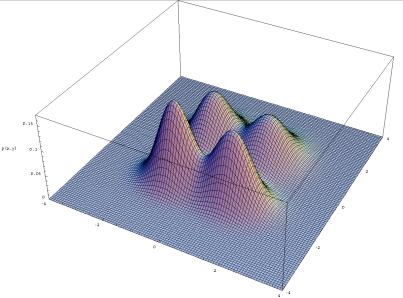
\includegraphics[width=0.7\linewidth]{Bimodal-bivariate-small.png}
\end{textblock*}

\end{frame}

\begin{frame}{混合分布}
\begin{itemize}
\item これまでは、全てのデータ$\bm{x}_i$ for $i=1,\ldots,N$を、
同じ一つの分布からdrawしていた
\begin{itemize}
\item 全ての確率変数$\bm{x}_i$ for $i=1,\ldots,N$が同じ分布に従うと考えていた
\end{itemize}
\item 一方、混合分布によるモデリングでは、同じ種類の分布だがパラメータの値が違うだけの分布を、$K$個用意する
\begin{itemize}
\item これらの分布をコンポーネントと呼ぶことがある
\end{itemize}
\item そして、各データ$\bm{x}_i$について、まず、カテゴリカル分布$\mbox{Cat}(\bm{\theta})$に従って
$K$個のコンポーネントから一つ選ぶ
\begin{itemize}
\item $\bm{\theta}=(\theta_1,\ldots,\theta_K)$はパラメータで、$\theta_k$は$k$番目の分布が選ばれる確率。
もちろん$\sum_k \theta_k = 1$が成り立つ
\end{itemize}
\item そして、$\bm{x}_i$がその選ばれた分布に従うと考える。
\end{itemize}
\end{frame}


\section{混合正規分布}

\begin{frame}\frametitle{Contents}
\Large \tableofcontents[currentsection]
\end{frame}

\begin{frame}{混合正規分布}
\begin{itemize}
\item 混合正規分布を使ったモデリングでは、データの集合$\{\bm{x}_1, \ldots, \bm{x}_N\}$が以下のように生成されると仮定する
\end{itemize}
\begin{enumerate}
\item $i$番目のデータ$\bm{x}_i$を生成するため、まず、カテゴリカル分布$\mbox{Cat}(\bm{\theta})$から、
確率変数$z_i$の値をdrawする
\begin{itemize}
\item 「$z_i = k$」は、$i$番目のデータについては$k$番目のコンポーネントが選ばれたことを意味する
\end{itemize}
\item その$z_i$の値に対応する確率分布から、$\bm{x}_i$をdrawする
\begin{align}
z_i & \sim \mbox{Cat}(\bm{\theta}) \notag \\
\bm{x}_i & \sim \mathcal{N}(\bm{\mu}_{z_i}, \bm{\Sigma}_{z_i})
\end{align}
\end{enumerate}
\end{frame}

\begin{frame}{単変量正規分布の混合分布の場合}
\begin{itemize}
\item $K$個のコンポーネントのなかから一つを選ぶ際に使われるカテゴリカル分布のパラメータは
$\bm{\theta} = (\theta_1,\ldots,\theta_K)$
\begin{itemize}
\item $\theta_k$は$k$番目のコンポーネントが選ばれる確率
\item $\sum_{k=1}^K \theta_k = 1$が成り立つ
\end{itemize}
\item $K$個の単変量正規分布をコンポーネントとして用意する
\item $k$番目の分布のパラメータは、平均$\mu_k$と標準偏差$\sigma_k$
\begin{itemize}
\item $k$番目のコンポーネントの確率密度関数は
\end{itemize}
\begin{align}
p(x;\mu_k,\sigma_k) = \frac{1}{\sqrt{2\pi\sigma_k^2}}\exp\Big( - \frac{(x - \mu_k)^2}{2\sigma_k^2} \Big)
\end{align}
\end{itemize}
\end{frame}

\begin{frame}{単変量正規分布の混合分布における同時分布}
\begin{itemize}
\item 単変量正規分布の混合分布によるモデリングでは、
データ集合$\{x_1, \ldots, x_N\}$と、コンポーネントへの所属を表す情報$\{z_1,\ldots,z_N\}$との、
同時分布が、以下のように得られる
\vspace{-.1in}
\begin{align}
& p( \{ x_1,\ldots,x_N \}, \{ z_1,\ldots,z_N \} ;\bm{\theta},\bm{\mu},\bm{\sigma})
= \prod_{i=1}^N p(x_i, z_i ; \theta_{z_i}, \sigma_{z_i}) \notag \\ &
= \prod_{i=1}^N \bigg[ \theta_{z_i} \times \frac{1}{\sqrt{2\pi\sigma_{z_i}^2}}\exp\bigg( - \frac{(x_i - \mu_{z_i})}{2\sigma_{z_i}^2} \bigg) \bigg]
\label{eq:joint_MN}
\end{align}
\begin{itemize}
\item 個々のデータは、(同じ分布からではないにせよ)独立に生成されると仮定している
\end{itemize}
\end{itemize}
\end{frame}


\section{混合正規分布:教師ありの場合}

\begin{frame}\frametitle{Contents}
\Large \tableofcontents[currentsection]
\end{frame}


\begin{frame}{教師ありの設定の場合 (1/2)}
\begin{itemize}
\item 教師ありの設定の場合、各データ$x_i$について、それがどのコンポーネントから生成されたかは、すでに分かっている
\item 言い換えれば、$z_i$の値も観測データに含まれる
\begin{itemize}
\item つまり、観測データを$\mathcal{D}$で表すとすると、$\mathcal{D} = \{ (x_1,z_1), \ldots, (x_N,z_N) \}$
($x_i$も$z_i$も、両方見えている)
\end{itemize}
\item このとき、式\eqref{eq:joint_MN}の同時分布が、そのまま、観測データ$\mathcal{D}$の尤度を表すことになる
\end{itemize}
\end{frame}

\begin{frame}{教師ありの設定の場合 (2/2)}
\begin{itemize}
\item そして、観測データ$\mathcal{D} = \{ (x_1,z_1), \ldots, (x_N,z_N) \}$の尤度は、下のように書き直すことができる
\vspace{-.15in}
\begin{align}
& p(\mathcal{D};\bm{\theta},\mu_1,\ldots,\mu_K,\sigma_1,\ldots,\sigma_K)
\notag \\ &
= \prod_{i=1}^N \bigg[ \theta_{z_i} \times \frac{1}{\sqrt{2\pi\sigma_{z_i}^2}}\exp\bigg( - \frac{(x_i - \mu_{z_i})}{2\sigma_{z_i}^2} \bigg) \bigg]
\notag \\ &
= \prod_{k=1}^K \bigg[ \theta_k^{c_k} \times \frac{1}{ (\sqrt{2\pi\sigma_k^2} )^{c_k}} 
\exp\bigg( - \frac{ \sum_{ \{ i : z_i = k \} } (x_i - \mu_k)^2 }{2\sigma_k^2} \bigg) \bigg]
\label{eq:likelihood_MN}
\end{align}
\vspace{-.15in}
\begin{itemize}
\item $c_k$は、$k$番目のコンポーネントから生成されたデータの個数
\end{itemize}
\end{itemize}
\end{frame}


\begin{frame}{教師ありの場合の混合正規分布の最尤推定}
\begin{itemize}
\item 混合正規分布のパラメータを、式\eqref{eq:likelihood_MN}の観測データの尤度を最大化することによって推定する方法を、以下に示す
\end{itemize}
\end{frame}


\begin{frame}
\FontMath
\vspace{.1in}
目的関数は
\begin{align}
& L(\bm{\theta},\mu_1,\ldots,\mu_K,\sigma_1,\ldots,\sigma_K)
= \ln p(\mathcal{D};\bm{\theta},\mu_1,\ldots,\mu_K,\sigma_1,\ldots,\sigma_K) 
+ \lambda \bigg( 1 - \sum_{k=1}^K \theta_k \bigg)
\notag \\ &
= \sum_{k=1}^K c_k \ln \theta_k - \sum_{k=1}^K c_k \ln \sigma_k
- \sum_{k=1}^K \frac{\sum_{ \{ i : z_i = k \} } (x_i - \mu_k)^2}{ 2\sigma_k^2} + \lambda \bigg( 1 - \sum_{k=1}^K \theta_k \bigg) + const.
\end{align}
目的関数$L$を、各パラメータで偏微分する。
\begin{align}
\frac{\partial L}{\partial \mu_k} = \frac{ \sum_{ \{ i : z_i = k \} } (x_i - \mu_k) }{\sigma_k^2}
= \frac{ \sum_{ \{ i : z_i = k \} } x_i - c_k \mu_k }{\sigma_k^2}
\end{align}
$\frac{\partial L}{\partial \mu_k} = 0$より、$\mu_k = \frac{ \sum_{ \{ i : z_i = k \} } x_i }{ c_k } = \bar{x}_k$を得る。
\begin{align}
\frac{\partial L}{\partial \sigma_k} = - \frac{c_k}{\sigma_k} + \frac{\sum_{ \{ i : z_i = k \} } (x_i - \mu_k)^2}{ \sigma_k^3}
\end{align}
$\frac{\partial L}{\partial \sigma_k} = 0$より、
$\sigma_k^2 = \frac{\sum_{ \{ i : z_i = k \} } (x_i - \bar{x}_k)^2}{ \sigma_k^2}$を得る。
\end{frame}

\begin{frame}
\FontMath
\begin{align}
\frac{\partial L}{\partial \theta_k} = \frac{c_k}{\theta_k} - \lambda \mbox{ , \ }
\frac{\partial L}{\partial \lambda} = 1 - \sum_{k=1}^K \theta_k
\end{align}
$\frac{\partial L}{\partial \theta_k} = 0$より、$\theta_k = \frac{c_k}{\lambda}$を得る。

$\frac{\partial L}{\partial \lambda} = 0$より、$1 - \sum_{k=1}^K \frac{c_k}{\lambda} = 0$を得る。

つまり、$\lambda = \sum_k c_k$が言えるので、$\theta_k = \frac{c_k}{\sum_k c_k}$を得る。

\

まとめると、
\begin{itemize}
\item $\theta_k$は、$k$番目のコンポーネントから生成されたデータの割合となる。
\item $\mu_k$と$\sigma_k$は、$k$番目のコンポーネントから生成されたデータだけの尤度をもとに最尤推定した値となる。
\end{itemize}
\end{frame}


\section{混合正規分布:教師なしの場合}

\begin{frame}\frametitle{Contents}
\Large \tableofcontents[currentsection]
\end{frame}


\begin{frame}{教師なしの設定の場合}
\vspace{-.05in}
\begin{itemize}
\item 教師なしの設定の場合、各データ$x_i$について、それがどのコンポーネントから生成されたかは、分からない!
\item $z_i$は、値が観測されない確率変数、すなわち潜在変数
\begin{itemize}
\item つまり、$\mathcal{D} = \{ x_1, \ldots, x_N \}$
\item 一方、潜在変数latent variablesの集合を$\mathcal{Z} = \{ z_1, \ldots, z_N \}$とする
\end{itemize}
\item このとき、下の$p(\mathcal{D}, \mathcal{Z})$は、観測データの尤度$p(\mathcal{D})$ではない
\vspace{-.13in}
\begin{align}
& p(\mathcal{D}, \mathcal{Z};\bm{\theta},\mu_1,\ldots,\mu_K,\sigma_1,\ldots,\sigma_K)
= \prod_{i=1}^N p(x_i, z_i ; \theta_{z_i}, \sigma_{z_i})
\notag \\ &
= \prod_{i=1}^N \bigg[ \theta_{z_i} \times \frac{1}{\sqrt{2\pi\sigma_{z_i}^2}}\exp\bigg( - \frac{(x_i - \mu_{z_i})}{2\sigma_{z_i}^2} \bigg) \bigg]
\end{align}
\end{itemize}
\end{frame}

\begin{frame}{観測データの尤度}
\vspace{-.05in}
\begin{itemize}
\item 潜在変数を含むモデリングの場合、観測データの尤度$p(\mathcal{D})$は、
潜在変数を周辺化して得られる
\begin{itemize}
\item $\mathcal{D}$を不完全データincomplete dataと呼ぶことがある
\end{itemize}
\begin{align}
p(\mathcal{D}) & = \sum_{\mathcal{Z}} p(\mathcal{D}, \mathcal{Z})
= \sum_{z_1=1}^K \sum_{z_2=1}^K \cdots \sum_{z_{N-1}=1}^K \sum_{z_N=1}^K p(\mathcal{D}, \mathcal{Z})
\notag \\ &
= \sum_{z_1=1}^K \sum_{z_2=1}^K \cdots \sum_{z_{N-1}=1}^K \sum_{z_N=1}^K \prod_{i=1}^N p(x_i, z_i)
\notag \\ &
= \prod_{i=1}^N \bigg( \sum_{z_i=1}^K p(x_i, z_i) \bigg)
\end{align}
\end{itemize}
\end{frame}

\begin{frame}{観測データの対数尤度}
\begin{itemize}
\item 混合正規分布の場合の観測データの対数尤度は、式\eqref{eq:joint_MN}より
\vspace{-.1in}
\begin{align}
& \ln p(\mathcal{D}) = \ln \sum_{\mathcal{Z}} p(\mathcal{D}, \mathcal{Z})
\notag \\ &
= \ln \sum_{z_1=1}^K \cdots \sum_{z_N=1}^K \bigg( \prod_{i=1}^N \bigg[ \theta_{z_i} \times \frac{1}{\sqrt{2\pi\sigma_{z_i}^2}}\exp\bigg( - \frac{(x_i - \mu_{z_i})}{2\sigma_{z_i}^2} \bigg) \bigg] \bigg)
\notag \\ &
= \ln \prod_{i=1}^N \bigg( \sum_{z_i=1}^K \bigg[ \theta_{z_i} \times \frac{1}{\sqrt{2\pi\sigma_{z_i}^2}}\exp\bigg( - \frac{(x_i - \mu_{z_i})}{2\sigma_{z_i}^2} \bigg) \bigg] \bigg)
\notag \\ &
= \sum_{i=1}^N \ln \bigg( \sum_{z_i=1}^K \bigg[ \theta_{z_i} \times \frac{1}{\sqrt{2\pi\sigma_{z_i}^2}}\exp\bigg( - \frac{(x_i - \mu_{z_i})}{2\sigma_{z_i}^2} \bigg) \bigg] \bigg)
\end{align}
\end{itemize}
\end{frame}

\begin{frame}{観測データの対数尤度の最大化}
\begin{itemize}
\item あとは、$\ln p(\mathcal{D})$を最大にする$\bm{\theta}=(\theta_1,\ldots,\theta_K)$や$\mu_1,\ldots,\mu_K$や$\sigma_1,\ldots,\sigma_K$を求めれば良い・・・???
\vspace{.3in}
\begin{itemize}
\item (偏微分の計算をしようとしてみると、問題がそう簡単ではなさそうであることに気づかれると思います。)
\end{itemize}
\end{itemize}
\end{frame}


\begin{frame}{積の対数と和の対数}
\begin{itemize}
\item 何かを掛け算したものの対数は、何かの対数の和に書き直せるので、扱いやすい
\begin{align}
\log(a \times b) = \log(a) + \log(b)
\end{align}
\item 何かを足し算したものの対数は、それ以上変形のしようがないので、扱いにくい
\begin{align}
\log(a + b) = \ldots
\end{align}\end{itemize}
\end{frame}

\begin{frame}{イェンセンの不等式(対数関数の場合)}
\begin{itemize}
\item $p_1,\ldots,p_K$を、$\sum_k p_k=1$を満たす正の実数とする
\item また、$x_1,\ldots, x_K$を正の実数とする
\item このとき、以下の不等式が成り立つ
\begin{align}
\ln \bigg( \sum_{k=1}^K p_k x_k \bigg) \geq \sum_{k=1}^K p_k \ln(x_k)
\end{align}
\begin{itemize}
\item 和の対数(扱いにくい!)の下界lower boundを、
対数の和(扱いやすい!)として得るため、イェンセンの不等式をよく使う
\item なお、対数関数に限らず、上に凸な関数なら、上の不等式は成立
\end{itemize}
\end{itemize}
\end{frame}



\end{document}